\section{Recolección}

%-------------------------------Recolección----------------------------------------------%

El proceso de recolección es parte fundamental del presente trabajo terminal, ya que permitió conformar el corpus utilizado en la etapa de entrenamiento, la Figura \ref{fig:etapRecoleccion} muestra las etapas que se desarrollaron durante el proceso de recolección.\\

\begin{figure}[H]
	\centering
	
\includegraphics[scale=.28]{imagenes/Capitulo5/etapasRecoleccion.png}
	\caption{Etapas de la recolección}
	\label{fig:etapRecoleccion}
\end{figure}

\Tlabel{cp5:sitiosWeb}
\subsection{Selección de sitios web}
\textit{Reuters Institute}\footnote{https://reutersinstitute.politics.ox.ac.uk/} realizó un informe anual para comprender como se consumen las noticias en distintos países, mediante el sitio \textit{YouGov}\footnote{https://mx.yougov.com/} se realizó la investigación utilizando cuestionarios en línea durante finales de enero y principios de febrero del año 2019. El informe reporto el índice de confianza que tienen los usuarios sobre los sitios noticiosos, la Figura \ref{fig:nivConfianza} muestra los sitios que tienen un mayor índice de confianza en una escala de 0 a 10.  

\begin{figure}[H]
  \centering
  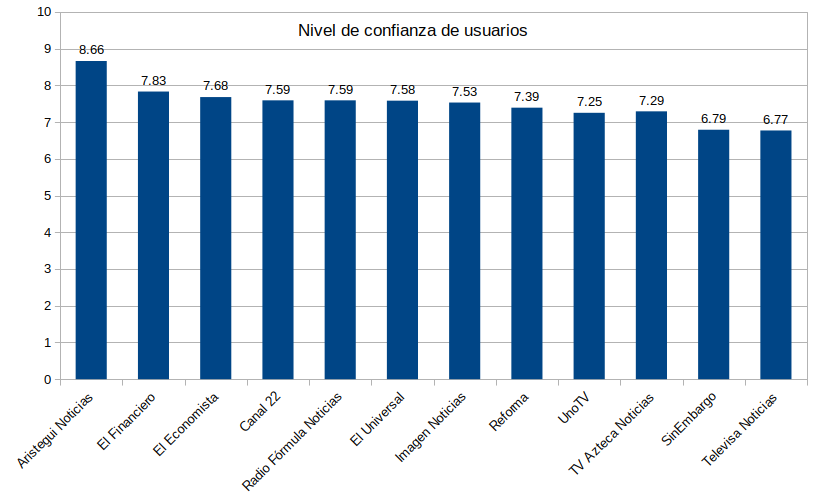
\includegraphics[scale=.4]{imagenes/Capitulo5/nivelConfianza.png}
  \caption{Nivel de confianza de usuarios al consultar un sitio web.}
  \label{fig:nivConfianza}
\end{figure}

El sitio web El Economista\footnote{https://www.eleconomista.com.mx/} contiene una sección llamada \textbf{Ranking de Medios Nativos Digitales}\footnote{https://www.eleconomista.com.mx/Ranking-de-Medios-Nativos-Digitales}, el cual muestra las estadísticas que realiza mes con mes acerca de los sitios de noticias web más consultados como se muestra en la Figura \ref{fig:rank}.\\

\begin{figure}[H]
  \centering
  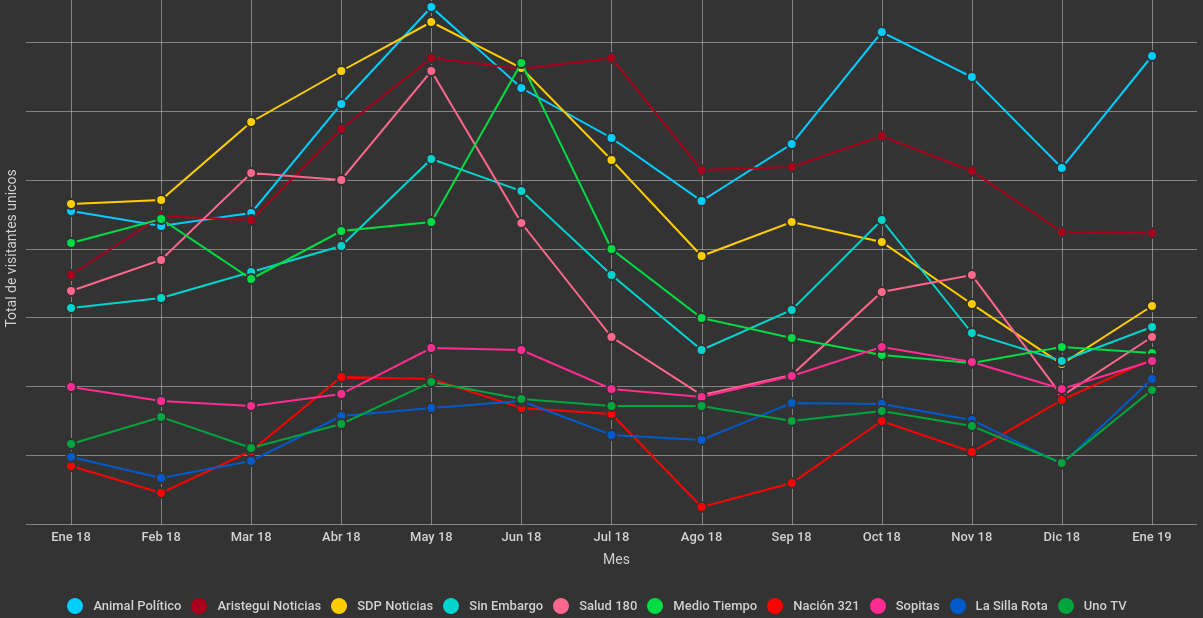
\includegraphics[scale=.25]{imagenes/Capitulo5/ranking.png}
  \caption{Ranking de sitios de noticias del periódo de enero del 2018 a enero del 2019.}
  \label{fig:rank}
\end{figure}

La compañía \textit{comScore}\footnote{https://www.comscore.com/} dedicada a proporcionar datos de marketing en Internet, en el año 2018 realizó un estudio en el cual indica los sitios web de noticias más visitados, los resultados se muestran en la Figura \ref{fig:comScore}.

\begin{figure}[H]
  \centering
  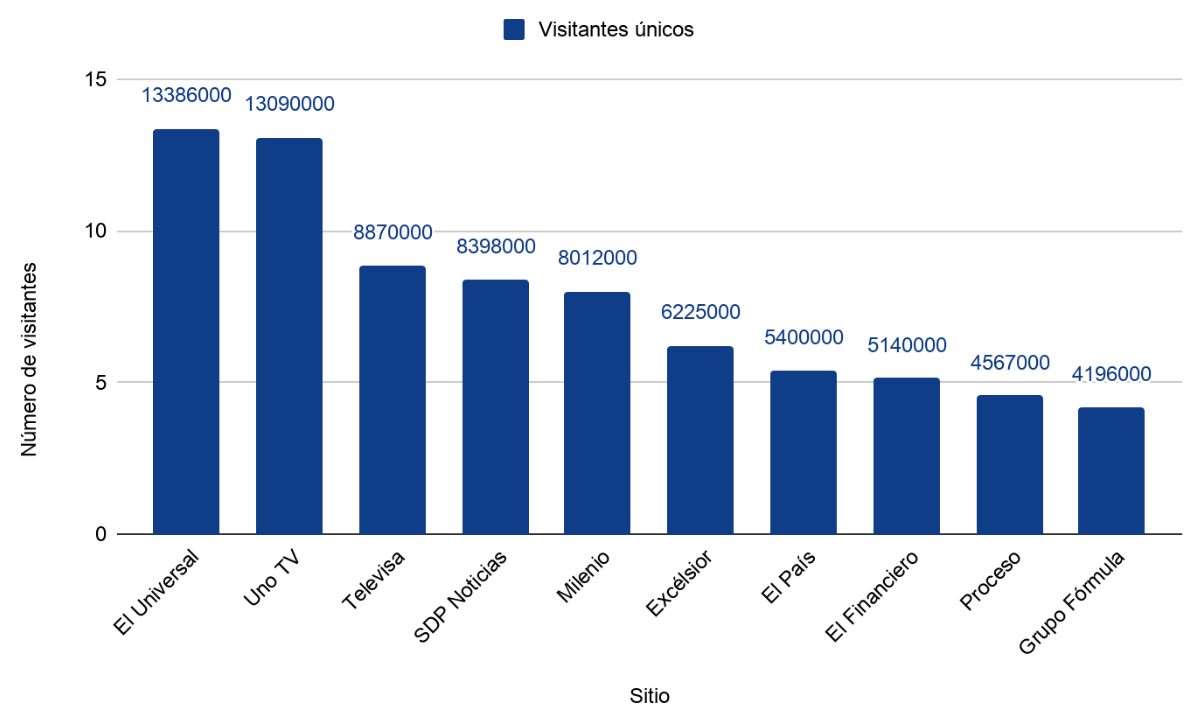
\includegraphics[scale=.32]{imagenes/Capitulo5/visitantesPorSitioComScore.png}
  \caption{Visitantes únicos a sitios de noticias durante el año 2018.}
  \label{fig:comScore}
\end{figure}

\Tlabel{c5:sitios}
Para llevar a cabo la selección de sitios web utilizados en el presente proyecto se realizó un análisis sobre aquellos que proveen de información noticiosa, entre los cuales se consideraron \textbf{foros de noticias}, \textbf{sitios de diarios} y \textbf{sitios de televisión}, en conjunto con las Figuras \textbf{\ref{fig:nivConfianza}}, \textbf{\ref{fig:comScore}}, \textbf{\ref{fig:rank}} se han seleccionado los sitios siguientes sitios:

\begin{itemize}

  \item \textbf{Aristegui Noticias}
  \item \textbf{El Economista}
  \item \textbf{La Jornada}
  \item \textbf{La Prensa}
  \item \textbf{Proceso}
  \item \textbf{Sopitas y TV Azteca}

\end{itemize}

De estas fuentes se recolectan noticias, ya que se desea obtener noticias de diversas fuentes de información, como lo son foros, blogs y sitios de televisoras.\\ 

Una vez definidos los sitios,  observamos que clasifican las noticias por secciones, lo cual permite una búsqueda más rápida de la información, la Tabla \ref{tabla:sitiosW}. muestra el análisis realizado a las secciones contenidas en los sitios seleccionados.
\\

\begin{table}[H]
\resizebox{\columnwidth}{!}{%
\begin{tabular}{|c|c|c|c|c|c|c|c|c|c|c|}
\hline
\rowcolor[HTML]{004784} 
\cellcolor[HTML]{004784}{\color[HTML]{EFEFEF} }                         & \multicolumn{10}{c|}{\cellcolor[HTML]{004784}{\color[HTML]{EFEFEF} Secciones}}                                                                                                                                                                                                                                                                                                                                                                                                                                                                                                                                    \\ \cline{2-11} 
\rowcolor[HTML]{004784} 
\multirow{-2}{*}{\cellcolor[HTML]{004784}{\color[HTML]{EFEFEF} Sitios}} & {\color[HTML]{EFEFEF} Nacional}                           & {\color[HTML]{EFEFEF} Internacional}                          & {\color[HTML]{EFEFEF} Ciudad}                             & {\color[HTML]{EFEFEF} Estados}                             & {\color[HTML]{EFEFEF} Economía}                            & {\color[HTML]{EFEFEF} Deportes} & {\color[HTML]{EFEFEF} Espectáculos} & {\color[HTML]{EFEFEF} Cultura}                                 & {\color[HTML]{EFEFEF} Política}                               & {\color[HTML]{EFEFEF} \begin{tabular}[c]{@{}c@{}}Ciencia y \\ tecnología\end{tabular}} \\ \hline
\begin{tabular}[c]{@{}c@{}}Aristegui\\ Noticias\end{tabular}            & México                                                    & Mundo                                                         & -                                                         & México                                                     & Economía                                                   & Deportes                        & -                                   & -                                                              & Poderes                                                       & -                                                                                      \\ \hline
\begin{tabular}[c]{@{}c@{}}Azteca\\ Noticias\end{tabular}               & -                                                         & Internacional                                                 & -                                                         & Estados                                                    & Finanzas                                                   & Deportes                        & Entretenimiento                     & -                                      & Política                                                      & Geek                                                                                   \\ \hline
El Economista                                                           & \begin{tabular}[c]{@{}c@{}}Urbes y\\ Estados\end{tabular} & \begin{tabular}[c]{@{}c@{}}The Washington\\ Post\end{tabular} & \begin{tabular}[c]{@{}c@{}}Urbes y\\ Estados\end{tabular} & \begin{tabular}[c]{@{}c@{}}Urbes y \\ Estados\end{tabular} & \begin{tabular}[c]{@{}c@{}}Valores y\\ Dinero\end{tabular} & DxT                             & -                                   & \begin{tabular}[c]{@{}c@{}}Artes, Ideas\\ y Gente\end{tabular} & \begin{tabular}[c]{@{}c@{}}Política y\\ Sociedad\end{tabular} & Tecnología                                                                             \\ \hline
La Jornada                                                              & -                                                         & Mundo                                                         & CDMX                                                      & Estados                                                    & Economía                                                   & Deportes                        & Espectáculos                        & Cultura                                                        & Política                                                      & Tecnología                                                                             \\ \hline
La Prensa                                                               & México                                                    & Mundo                                                         & Metrópoli                                                 & República                                                  & -                                                          & Deportes                        & Gossip                              & Cultura                                                        & México                                                        & Tecnología                                                                             \\ \hline
Proceso                                                                 & Nacional                                                  & Internacional                                                 & La Capital                                                & Estados                                                    & -                                                          & Deportes                        & Miscelánea                          & Cultura                                                        & Política                                                      & Tecnología                                                                             \\ \hline
Sopitas                                                                 & Noticias                                                  & -                                                             & -                                                         & -                                                          & -                                                          & Deportes                        & En el show                          & -                                                              & -                                                             & Geek                                                                                   \\ \hline
\end{tabular}
}
\caption[Secciones de los sitios web]{Secciones existentes en los sitios web}
\label{tabla:sitiosW}
\end{table}

Una vez que se analizaron las secciones con las que contaba cada sitio, se procedió a homologar las secciones en las cuales la mayoría de los sitios coincidian, por lo cual se quedarón definidas 5 secciones para clasificación de las noticias:

\begin{itemize}
    \item \textbf{Política}
    \item \textbf{Deportes}
    \item \textbf{Ciencia y tecnología}
    \item \textbf{Economía}
    \item \textbf{Cultura}
\end{itemize}

Cabe mencionar que hay muy pocos sitios que publican noticias de la sección \textbf{Ciencia y tecnología} y \textbf{Cultura}, por ello se consideraron éstas secciones.

%------------------------------------------- Listo
\subsection{Análisis de sitios web}

Una vez definida la información requerida de cada noticia se realizó un análisis sobre la estructura \textbf{XML} (\textit{Extensible Markup Language}, por sus siglas en inglés), con el fin de realizar expresiones \textit{XPath} que permiten recorrer y procesar un documento XML, dado que cada sitio web cuenta con una estructura diferente, ha sido necesario realizar el análisis individual. Cabe mencionar que existen sitios los cuales realizan actualizaciones a su página, por esta razón cada dos meses se analizaban, con el fin de verificar que la estructura XML no cambiará.\\

Una expresión \textit{XPath} de ruta permite buscar y seleccionar los distintos nodos de un documento XML. En el siguiente Cuadro \ref{box:xmlEjemplo} se muestra un ejemplo con los elementos de una nota, los cuales son: \textbf{para}, \textbf{de}, \textbf{titulo}, \textbf{texto}, en un documento XML estos son los nodos que conforman una nota.\\

\begin{mygraybox}[label={box:xmlEjemplo}]{Documento XML}
\begin{tabbing}
<nota> \= \\\kill
\>	<para>Daniel</para>\\
\>	<de>Andres</de>\\
\>	<titulo>Recordatorio</titulo>\\
\>	<texto>Recuerda despertar temprano.</texto>\\
</nota>
\end{tabbing}
\end{mygraybox}
\ \\
La expresión \textit{XPath} que permite extraer el contenido de la etiqueta \textbf{<texto> </texto>} se muestra en el Cuadro \ref{box:xpathEjemplo}: \\

\begin{mygraybox}[label={box:xpathEjemplo}]{Expresión XPath} 
\textbf{/nota/texto/text()}
\end{mygraybox}

Para cada sitio web se crearon expresiones \textit{XPath} para recolectar el contenido.

%------------------------------------------- Listo
\subsection{Creación de recolector}

Como se explicó en el capítulo 3 (ver \Tref{c3:crawler}{Crawler}) un \textit{Crawler} permite descargar información de una página web, como se muestra en la Figura \ref{Fig:recoleccion}. La implementación en el trabajo terminal ha requerido diseñar 7 recolectores, uno por cada sitio web (ver \Tref{c5:sitios}{sitios web}). \\

\begin{figure}[H]
	\centering
	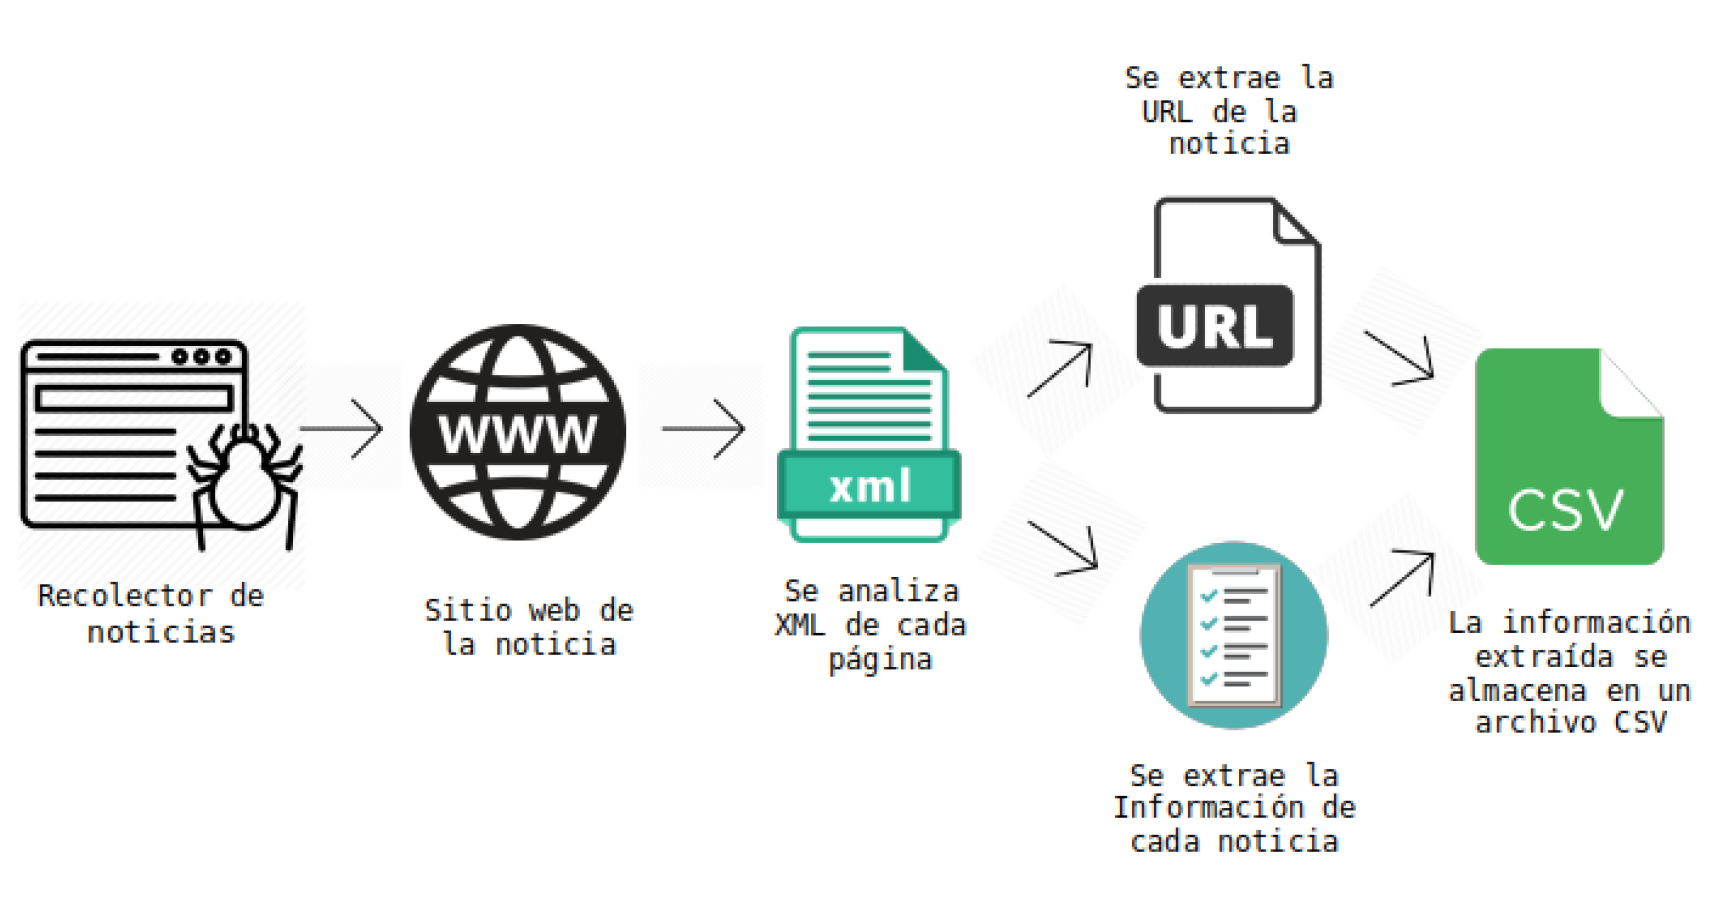
\includegraphics[scale=.3]{imagenes/Capitulo5/recoleccion.png}
	\caption{Proceso de recolección}
	\label{Fig:recoleccion}
\end{figure}

El desarrollo del presente trabajo terminal se ha realizado en sistema operativo \textit{Linux} en su distribución Ubuntu, paa realizar la creación de los recolectores se ha utilizado el lenguaje de programación \textbf{Python 3}\footnote{https://www.python.org/}, en conjunto con \textbf{Scrapy}\footnote{https://scrapy.org/}, Fsramework que permite la extracción de información de sitios web. 

La información que ha sido recuperada de las noticias se muestra a continuación:
\begin{itemize}
	\item \textbf{URL}: La dirección web donde se encuentra localizada la noticia 
	\item \textbf{TÍtulo}: Encabezado de la noticia recolectada
	\item \textbf{Autor}: Es el nombre de la persona que redacto la noticia o el nombre de la editorial
	\item \textbf{Fecha}: Es la fecha en la cual la noticia ha sido publicada
	\item \textbf{Descripción}: Es una idea general del contenido de la noticia. Cabe mencionar que no todas las noticias cuentan con una descripción
	\item \textbf{Noticia}: Es la redacción realizada por el autor acerca de la noticia. Es de relevancia mencionar que este elemento más importante de los artículos decargados 
\end{itemize}

Cada uno de los recolectores contenia expresiones \textit{XPath} que permitían recolectar la información de cada noticia, el Cuadro \ref{box:crawlerEjemplo} muestra un ejemplo de las expresiones \textit{XPath} utilizadas para recolectar noticias del sitio web Aristegui Noticias\footnote{https://aristeguinoticias.com/}\\

\begin{mygraybox}[label={box:crawlerEjemplo}]{Ejemplo de expresiones \textit{XPath} del sitio Aristegui Noticias}
\begin{small}
\begin{verbatim}
url= url
titulo = //div[@class="class_subtitular"]/h1/text()
autor = //div[@class="share_nom"]/text()
fecha = //div[@class="share_publicado"]/text()
descripcion = //div[@class="class_text2"]/text())
noticia = //div[@class="class_text"]/p/child::node()/text()
\end{verbatim}
\end{small}
\end{mygraybox}
\ \\
Cabe destacar que las noticias recolectadas se almacenaron en un archivo \textbf{CSV} (\textit{comma separeted values}, por sus siglas en inglés), con la estructura que se muestra en la Tabla \ref{tab:csv}, donde la primera fila (Encabezado) define los elementos de este archivo, además las filas consecuentes representan el contenido recolectado de cada noticia.\\

%\begin{mygraybox}[label={box:csv}]{Encabezado de un archivo CSV}
\begin{table}[H]
\centering
\resizebox{\columnwidth}{!}{
\begin{tabular}{|c |c |c |c |c |c |c}
\hline
\textbf{url}& \textbf{título}& \textbf{autor}& \textbf{fecha}& \textbf{descripción}& \textbf{noticia}\\
\cline{1-6}
url ejemplo 1& título ejemplo 1& autor ejemplo 1& fecha ejemplo 1& descripción ejemplo 1& noticia ejemplo1\\
\hline
url ejemplo 2& título ejemplo 2& autor ejemplo 2& fecha ejemplo 2& descripción ejemplo 2& noticia ejemplo2\\
\hline
\end{tabular}
}
\caption{Ejemplo de estructura de un archivo CSV}
\label{tab:csv}
\end{table}
%\end{mygraybox}

\subsection{Recolección de noticias}

Para el desarrollo de esta etapa, se recolectaron noticias de las secciones: \textbf{ciencia y tecnología}, \textbf{cultura}, \textbf{deportes}, \textbf{economía} y \textbf{política}, de los sitios web \textbf{Aristegui Noticias}, \textbf{El Economista}, \textbf{La Jornada}, \textbf{La Prensa}, \textbf{Proceso}, \textbf{Sopitas} y \textbf{TV Azteca}, durante el periodo de julio a septiembre del año 2019, cada cuatro días, con el fin de no tener noticias repetidas. El almacenamiento de las noticias se realizó en un directorio por sección, dentro de cada uno de estos se guardaban las noticias recolectadas por sitio web.\\

Una vez finalizada la primera etapa de recolección, los resultados obtenidos por sección se muestran en la Figura  \ref{Fig:notseccionV1}.
%Mencionar como nombre primer corte de recolección y poner numero de noticias
\begin{figure}[H]
	\centering
	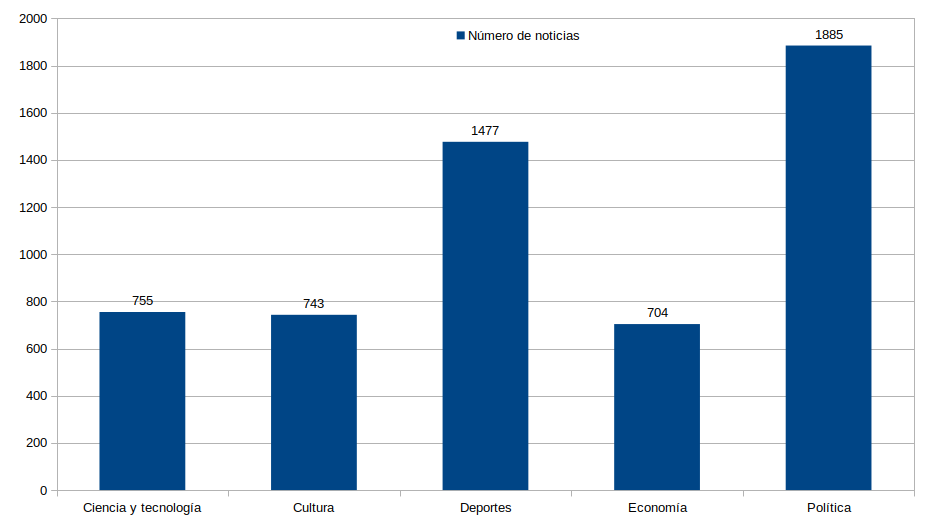
\includegraphics[scale=.4]{imagenes/Capitulo5/noticiasPorSeccionV1.png}
	\caption{Noticias recolectadas durante el primer corte.}
	\label{Fig:notseccionV1}
\end{figure}

Cabe destacar que el número de noticias recolectado durante el primer corte, no se encontraba balanceado, es decir el número de noticias por sección era distinto, por ello se decidió continuar con el proceso de recolección de noticias, con el fin de balancear el corpus.\\
Una vez finalizada la segunda etapa de recolección el número de noticias se muestra en la Figura \ref{Fig:notseccion} 

\begin{figure}[H]
	\centering
	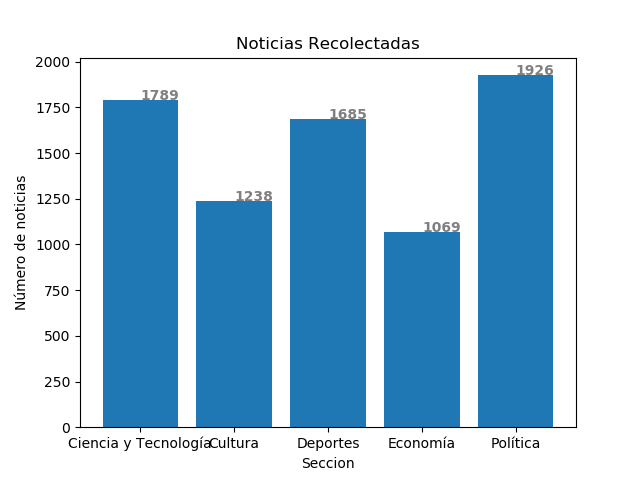
\includegraphics[scale=.42]{imagenes/Capitulo5/noticiasPorSeccionV2.png}
	\caption{Noticias recolectadas al finalizar el segundo corte.}
	\label{Fig:notseccion}
\end{figure}

Los resultados que obtuvimos por sitio web se muestran en la Figura \ref{Fig:notPorSit} 

\begin{figure}[H]
	\centering
	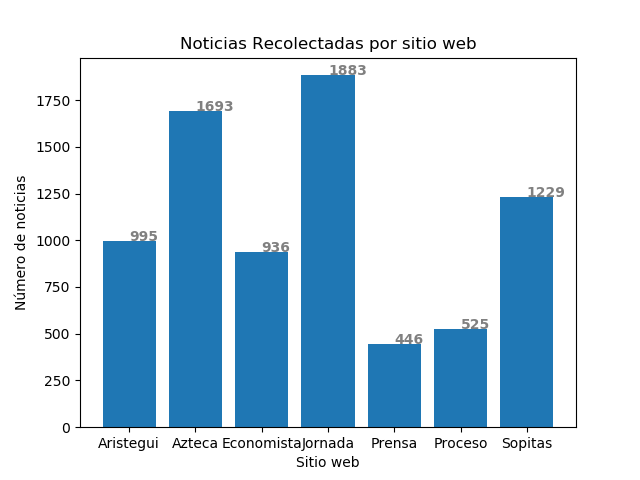
\includegraphics[scale=.45]{imagenes/Capitulo5/noticiasPorSitio.png}
	\caption{Noticias recolectadas por sitio web al finalizar el segundo corte}
	\label{Fig:notPorSit}
\end{figure}

Una vez concluida la recolección de noticias, se eliminaron aquellas noticias que se encontraban más de una vez dentro de los archivos, utilizando listas en \textbf{Python} en el cual se validaba la URL de la noticia no se encontrará en la lista. Cabe mencionar que existían noticias que contenían \textit{tuits} redactados en lenguaje inglés, por esta razón se procedió a eliminar el contenido de este idioma. Al concluir este proceso se obtuvo un total de 7,707 artículos. La Figura  \ref{fig:cp5:secciones} muestra el total de noticias por sección y la Tabla \ \ref{tabla:numNotic} muestra las noticias recuperadas por cada sitio web.




\begin{figure}[h]
  \centering
  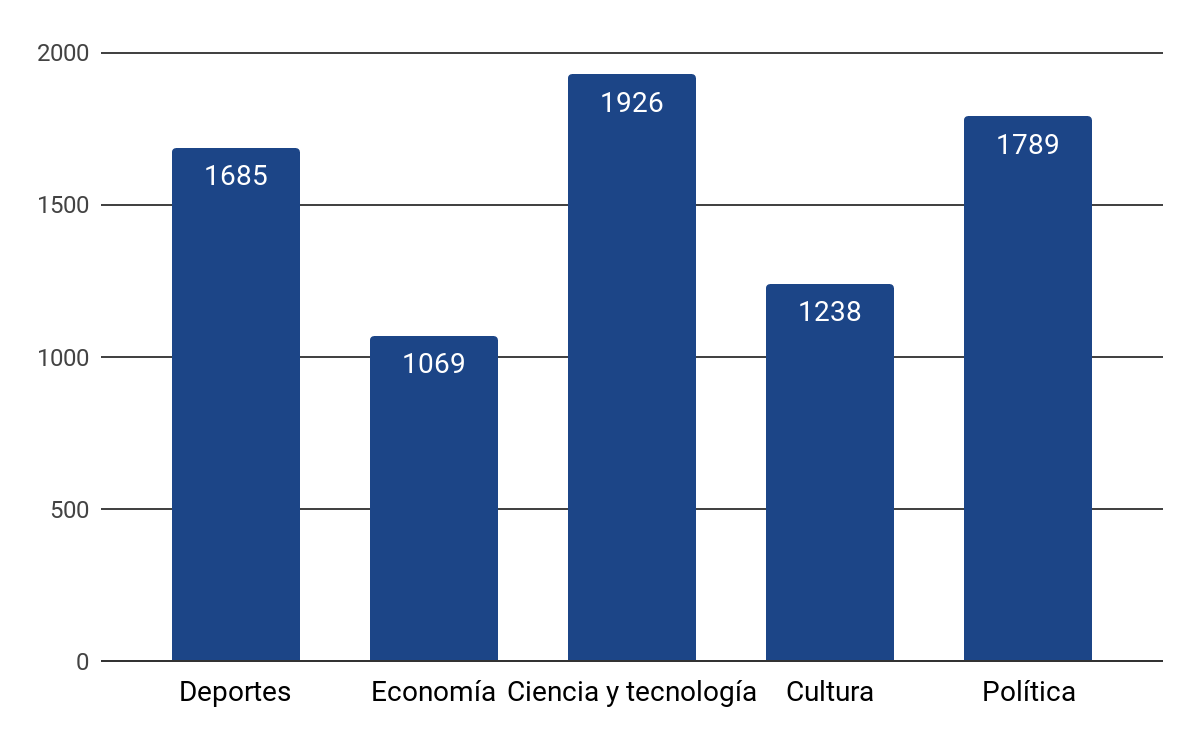
\includegraphics[scale=.28]{imagenes/Capitulo5/seccionesCr.png}
  \caption{Noticias recolectadas secciones}
  \label{fig:cp5:secciones}
\end{figure}


%
%\begin{table}[H]
%\centering
%  \begin{tabular}{|l|c|}
%  %-----------------------Ecanbezado-----------------------------------%
%    \hline
%\multicolumn{1}{| >{\columncolor{myBlueChapter}}l|}{ \textcolor{myWhite}{\textbf{Sección}} }&
%\multicolumn{1}{| >{\columncolor{myBlueChapter}}l|}{ \textcolor{myWhite}{\textbf{Número de noticias%}} }%
%\\  %\cline{1-2}%
%  %-%-------------%
%
%Deportes& 1685\\
%\hline
%Economía& 1069\\
%\hline
%Política& 1926\\
%\hline
%Cultura& 1238\\
%\hline
%Ciencia y Tecnología& 1789\\
%\hline
%  \end{tabular}
%\caption{Número de noticias}
%\label{tabla:totalSeccion}
%\end{table}

%--------------------------------------------------------------------------------%
\begin{table}[H]
\centering
\begin{tabular}{|l|l|c|}
\hline
 \multicolumn{1}{| >{\columncolor{myBlueChapter}}c|}{ \textcolor{myWhite}{\textbf{Sitio}} }
&\multicolumn{1}{| >{\columncolor{myBlueChapter}}c|}{ \textcolor{myWhite}{\textbf{Sección  }} }
&\multicolumn{1}{| >{\columncolor{myBlueChapter}}c|}{ \textcolor{myWhite}{\textbf{Número de Noticias}} }
\\ \cline{1-3}

\multirow{5}{*}{\textbf{Aristegui Noticias}} & Ciencia y Tecnología & 99                 \\ \cline{2-3} 
                                    & Cultura              & 179                \\ \cline{2-3} 
                                    & Deportes             & 308                \\ \cline{2-3} 
                                    & Economía             & 161                \\ \cline{2-3} 
                                    & Política             & 248                \\ \hline
\multirow{5}{*}{\textbf{Azteca Noticias}}& Ciencia y Tecnología & 986           \\ \cline{2-3} 
                                    & Cultura              & 0                  \\ \cline{2-3} 
                                    & Deportes             & 280                \\ \cline{2-3} 
                                    & Economía             & 77                 \\ \cline{2-3} 
                                    & Política             & 350                \\ \hline
\multirow{5}{*}{\textbf{El Economista}}& Ciencia y Tecnología & 18              \\ \cline{2-3} 
                                    & Cultura              & 267                \\ \cline{2-3} 
                                    & Deportes             & 214                \\ \cline{2-3} 
                                    & Economía             & 201                \\ \cline{2-3} 
                                    & Política             & 236                \\ \hline
\multirow{5}{*}{\textbf{La Jornada}}& Ciencia y Tecnología & 4                  \\ \cline{2-3} 
                                    & Cultura              & 424                \\ \cline{2-3} 
                                    & Deportes             & 284                \\ \cline{2-3} 
                                    & Economía             & 512                \\ \cline{2-3} 
                                    & Política             & 659                \\ \hline
\multirow{5}{*}{\textbf{La Prensa}} & Ciencia y Tecnología & 68                 \\ \cline{2-3} 
                                    & Cultura              & 90                 \\ \cline{2-3} 
                                    & Deportes             & 93                 \\ \cline{2-3} 
                                    & Economía             & 118                \\ \cline{2-3} 
                                    & Política             & 77                 \\ \hline
\multirow{5}{*}{\textbf{Proceso}}   & Ciencia y Tecnología & 65                 \\ \cline{2-3} 
                                    & Cultura              & 13                 \\ \cline{2-3} 
                                    & Deportes             & 335                \\ \cline{2-3} 
                                    & Economía             & 0                  \\ \cline{2-3} 
                                    & Política             & 112                \\ \hline
\multirow{5}{*}{\textbf{Sopitas}}   & Ciencia y Tecnología & 549                \\ \cline{2-3} 
                                    & Cultura              & 265                \\ \cline{2-3} 
                                    & Deportes             & 171                \\ \cline{2-3} 
                                    & Economía             & 0                  \\ \cline{2-3} 
                                    & Política             & 244                \\ \hline
\end{tabular}
\caption[Noticias recolectadas por sitio web]{Número de noticias recolectadas por sección de los sitios web}
\label{tabla:numNotic}
\end{table}



